\documentclass{scrartcl}

\usepackage{siunitx}
\usepackage{graphicx}
\usepackage{caption}
\usepackage{glossaries}
\usepackage[english]{babel}
\usepackage{booktabs}
\usepackage[linktoc=all,hidelinks]{hyperref}
\usepackage{fontspec}
% \usepackage{authblk}
\usepackage{unicode-math}

% \makeatletter
% \renewcommand\AB@affilsepx{,~ \protect\Affilfont}
% \makeatother

\setkomafont{author}{\sffamily}

\newcommand{\nump}[2]{\num[round-mode=places,round-precision=#2]{#1}}
\DeclareGraphicsExtensions{.pdf,.eps}
\bibliographystyle{unsrt}

\title{Report}
\subtitle{A study of machine learning algorithms for reconstruction of missing energy in particle physics experiments.}
% \subject{Statistical Machine Learning}

\author{
  Max Isacson, \url{max.isacson@physics.uu.se}
  \and
  Mikael M\aa rtensson, \url{mikael.martensson@physics.uu.se}
  \and
  Camila Rangel Smith, \url{camila.rangel@physics.uu.se}
  \and
  Henrik Öhman, \url{ohman@cern.ch}
}
% \author[1]{Max Isacsson}
% \author[2]{Mikael M\aa rtensson}
% \author[3]{Camila Rangel Smith}
% \author[4]{Henrik \"{O}hman}
% \affil[1]{\small\url{max.isacsson@physics.uu.se}}
% \affil[2]{\url{mikael.martensson@physics.uu.se}}
% \affil[3]{\url{camila.rangel@physics.uu.se}}
% \affil[4]{\url{ohman@cern.ch}}

\newacronym{ANN}{ANN}{Artificial Neural Network}
\newacronym{ML}{ML}{Machine Learning}

\newcommand{\etmiss}{$E_\mathrm{T}^\text{miss}$}
\newcommand{\exmiss}{$E_x^\text{miss}$}
\newcommand{\eymiss}{$E_y^\text{miss}$}
\newcommand{\pt}{\ensuremath{p_\text{T}}~}
\newcommand{\mt}{\ensuremath{M_\text{T}}~}

\begin{document}
\maketitle

% \begin{figure}
%     \centering
%     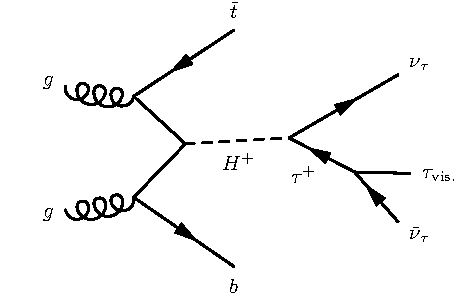
\includegraphics[width=.7\textwidth]{fig/heavyHplustaunu4fs.pdf}
%     \caption{Feynman diagram of the production and decay of a charged Higgs boson. Not shown is the hadronic top decay $\bar t \to \bar b W^-(q \bar q')$.}\label{fig:hplus}
% \end{figure}

\section{Introduction and Objective}

\section{The Dataset}
\subsection{Structure}
The dataset consists of simulated $pp$ collision events, in which a charged Higgs is produced and decays as $H^+\to\tau\nu$. Each event is described by one set of observable variables and one set of unobservable variables.

Observable variables:
\begin{itemize}
    \item \exmiss, \eymiss --- The $x$- and $y$-components of the missing energy.
    \item $P_{\tau_\mathrm{vis.}}$ --- The 4-momentum of the visible (hadronic) part of the $\tau$ decay.
    \item $P_{b_0}$, $P_{b_1}$, $P_{q_0}$, $P_{q_1}$ --- The 4-momenta of the two $b$-jets and two light jets.
\end{itemize}

Unobservable variables:
\begin{itemize}
    \item $P_{\nu_\tau}$ --- The 4-momentum of the neutrino from the charged Higgs decay.
    \item $P_{\bar\nu_\tau}$ --- The 4-momentum of the neutrino from the $\tau$ decay.
\end{itemize}

\subsection{Production}
MG5\_aMC@NLO \cite{Alwall:2014hca} is used for the matrix element computation of $gg / q \bar q \to H^+$ and the event simulation. The events are then passed to PYTHIA8 \cite{Sjöstrand2015159} for the showering and hadronization, and for the $H^+\to \tau\nu$ decay. Finally, the detector response is simulated using DELPHES \cite{Favereau2014} with an ATLAS-like geometry.

\subsection{Estimated and true quantities}
The true quantities for both the observable and the unobservable variables are available as output from the event simulation. The estimated values for the observable variables are reconstructed from the output from the detector response simulation.

\section{Methods and Implementation}

\subsection{Predictor selection}

\subsection{Artificial Neural Network}

The data needs to be scaled to avoid the tails of the \gls{ANN} activation functions and improve the learning rate. The method used here is to scale it such that the minimum is -1 and the maximum is 1 for each training set variable. The test set data is scaled using the scaling parameters computed from the training set. Another scaling method would be to scale the mean to 0 and the standard deviation to 1, but this was found to slow down the training and give worst result.

The \gls{ANN} implemented here uses Python with SciPy \cite{scipy}, Numpy \cite{numpy}, and Pandas \cite{pandas} for general data processing, and Keras \cite{keras} for the actual neural network. The number of input nodes is restricted to the 19 selected predictor variables and the output to the target dimension of 1. Since the network is used for regression, the activation functions between the last hidden layer and the output must be linear.

Training is performed using stochastic gradient descent with the Nesterov method \cite{nesterov} and a mean-squared-error loss function. The learning rate was set to 0.1, the learning rate decay to $\num{1e-6}$, and the momentum to 0.9.

A large number of configurations of the hidden layers were tested by varying the number of layers, the number of perceptrons in each layer, and the activation functions (sigmoid, tanh, and softmax). Sigmoid activation functions produced the best result for a fixed training period. A network with two hidden layers (i.e. 4 layers counting the 19 node input layer and 1 node output layer) with 25 and 10 perceptrons was found to be sufficiently complex. Using deeper networks, e.g. one with 4 hidden layer with 20, 35, 25, and 15 perceptrons, did not improve the result.

\subsection{Support Vector Regression}

Support vector machines can be used for regression, and the method is then called support vector regression (SVR). It employs two slack variables, $ξ_n ≥ 0$ and $\hat{ξ}_n ≥ 0$ and the corresponding error function to minimize is
\[
  C \sum_{n=1}^N(ξ_n + \hat{ξ}_n) + \frac{1}{2}||w||^2
\]
where $C$ is the cost variable. The implementation used is the \texttt{SVR} class from \texttt{scikit-learn}, and it is an $ε$-SVR method. This implementation has four built-in kernels: RBF, sigmoid, linear, and polynomial. The selected predictors in the dataset are scaled to have a mean of 0 and a variance of 1 using the \texttt{StandardScaler} class from \texttt{scikit-learn}.

With the presented dataset, the selected SVR algorithm is not converging within a few minutes runnning time. The maximum number of iterations is therefore limited to 1000. A greater number of iterations is not found to yield significantly better results. The kernel that performs best is the RBF kernel. The value of the cost function is by default set to 1.0, but this setting yields a very poor resolution. Different values of the cost function are tested, and a value of $C=100.0$ is found to be (near) optimal. For the soft margin the default value of $ε=0.1$ is good.

Regardless of the choice of $C$ and $ε$, the performance of the SVR is found to be no better than that of linear ridge regression. The resolution is not improved, and the shape of the true and reconstructed transverse component of the missing energy is not recovered by the prediction.

\subsection{Trees and forests}

Decision trees and ensemble methods, and in particular boosted decision trees (BDTs), have been a popular choice of method in particle physics. The method of decision trees are based on using multiple discriminating variables, and multiple choices in a binary tree, to find the prediction that best describes the target variable. When using ensemble methods, such as extra trees, gradient boosting, or random forests multiple such trees are created, each with its own weight describing its "importance". The tree depth plays an important role when considering the trade-off between over-training and bias, and with the ensemble methods the number of trees is also an important parameter.

The performances of the classes \texttt{DecisionTreeRegressor}, \texttt{ExtraTreesRegressor}, \texttt{GradientBoostingRegressor}, and \texttt{RandomForestRegressor} in \texttt{scikit-learn} are examined. Different settings for the tree depth and (for the ensemble methods) number of trees are used. Near optimal values for the depth and the number of trees is found to be 15 and 100 for all methods and all ensemble methods respectively. The decision tree regression shows some improvement in resolution, but the shape of the transverse component of the missing energy is not recovered by the prediction. Neither in the ensemble methods is the shape of the missing energy recovered, but the resolution is improved. All three ensemble method show similar performance.

\section{Results}
\label{sec:results}

% Please describe how the missing mass is calculated

\section{Discussion}

Out of all the \gls{ML} methods tried, \gls{ANN} showed the best performance in terms of resolution and predicting the \pt of the tau neutrino.

This project focused on predicting the transverse momentum \pt of the tau neutrino $\nu_\tau$ by using the reconstructed four-momenta and missing energy seen by the detector as input and training on the true \pt given by the Monte-Carlo simulation. In the end it is the mass of the $H^+$ that is interesting, which means that one option is to target the $H^+$ mass directly. This would require Monte-Carlo for a range of possible $H^+$ masses (3 mass-points were used in this study). Another option is to target the complete three-vector of the missing energy or the (combined or separate) four-vectors of the two neutrinos. These options were briefly looked at but were considered to be out of the scope of this project. They will be pursued in more detail in future studies.

To compute the missing transverse mass \mt (described in sec. \ref{sec:results}) from the \pt predicted by the \gls{ML} methods, the angle $\phi$ of the \pt is needed. However, since we are only predicting the \pt, the angle $\phi$ is unknown and is instead taken from the angle of \mt. It would have been better to also predict $\phi$. This will also be studied in the future.

% Mention that we use phi(met) when calculating the mT for the prediction. In principle we should predict phi as well. 
% The second nu as source of error

\bibliography{refs}

\end{document}
